\documentclass[a4paper,12pt]{article}
\usepackage[T1]{fontenc}
\usepackage[french]{babel}
\usepackage{graphicx}
\author{Thomas Bretecher}
\title{Simulation d'une population de fourmis}

\begin{document}

\maketitle

\section{Utilisation}

Le programme \verb|fourmis.py| simule une population de fourmis, leurs déplacements sur une grille, en prenant en compte l'accès à la nourriture dans l'environnement.

Les différentes options sont :

\begin{description}   

\item \verb|-f, --fourmis| Le nombre de fourmis, 20 par défaut.

\item \verb|-n, --nb-nourriture| Le nombre de points de nourriture, 10 par défaut.

\item \verb|-v, --pv-max| Le nombre de points de vie des fourmis au début de la simulation, 20 par défaut.

\item \verb|-t, --tours| Le nombre de tours avant l'arrêt de la simulation, 20 par défaut.

\item \verb|-p, --trophallaxie| Active le partage de nourriture entre les fourmis.

\item \verb|-g, --graphique| Désactive l'affichage graphique.

\end{description}

Par exemple la commande \verb|fourmis.py -f 30 -p -n 15| exécuterait une simulation avec 30 fourmis, 15 points de nourriture, et le partage de nourriture entre les fourmis.

Pendant l'exécution, l'affichage graphique pourrait ressembler à ceci :

\begin{center}
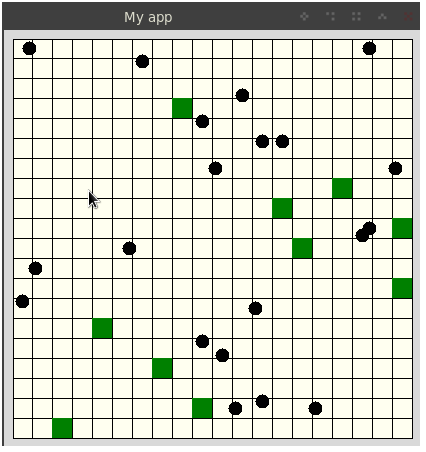
\includegraphics[scale=0.34]{fourmis.png}
\end{center}

\section{Méthode}

Pour réaliser le programme, la première étape a été d'identifier les variables nécessaires. Elles rentraient dans deux catégories : les paramètres de la simulation entrées en début d'exécution, et les données créées et manipulées au cours de la simulation. Ces dernières sont la position et le nombre de points de vie des différentes fourmies, et la position des points de nourriture.
La structure pour les positions des fourmies et des points de nourriture, et pour les points de vie, était imposée par le module \verb|ant_animate| fourni pour l'affichage graphique.

Ensuite, la seconde étape a été la réalisation d'un premier prototype implémentant les fonctionnalités essentielles : déplacement des fourmis, recharge des points de vie quand sur un point de nourriture, mort des fourmis. Une fois ce prototype réalisé, le code a été versionné à l'aide de \verb|git| (https://github.com/tbretecher/fourmis).

Après ça, les autres fonctionnalités ont été implémentées : la trophallaxie, détaillée dans la section 4; les arguments en ligne de commande, avec le module \verb|argparse|; les fonctions d'initialisation des structures de données; et la modification du format des coordonnés.

Le format imposé par \verb|ant_animate| pour les coordonées ne me convenait pas. En effet, il imposait d'utiliser des variables \verb|x| et \verb|y| séparées, alors qu'il me semblait qu'en les stockant dans une \emph{tuple} \verb|(x, y)|, je pouvais simplifier mon code. De même, le module utilise des coordonées comprises entre 1 et 20, alors que le passage d'un bord à l'autre de la grille était beaucoup plus simple avec des coordonées comprises entre 0 et 19. J'ai donc légèrement modifié \verb|ant_animate| pour pouvoir utiliser ces structures de données.

Enfin, \verb|fourmis.py| a régulièrement été passée dans l'outil \verb|pylint|, qui vérifie la qualité du code (principalement le style du code).

\section{Structures de données}

Le programme s'organise autour de deux objets, \verb|food| et \verb|d_fourmis|.

Tout d'abord, \verb|d_fourmis| est un dictionnaire dont les clefs sont les numéros attribués à chaque fourmis. Puis, pour chacune des fourmis, un second dictionnaire est imbriqué, dont les clefs sont \verb|coords| et \verb|food|.

\verb|coords| contient une liste de coordonées, correspondants aux coordonées de la fourmi en question à chaque tour de la simulation. À chaque tour, une nouvelle coordonée est ajoutée à la liste. Celles-ci sont représentées par des tuples de deux valeurs entre 0 et 19, par exemple \verb|(5, 13)|.

\verb|life| contient une liste d'entiers, qui représente les points de vie de la fourmie à chaque tour. Le premier élément de la liste, qui correspond au début de la simulation, contient donc le nombre de points de vie défini au lancement de la simulation, puis comme pour \verb|coords|, une nouvelle valeur est ajoutée à chaque tour.

Voici un exemple de \verb|d_fourmis| en fin de simulation, avec 3 fourmis et 5 tours de simulation :

\begin{verbatim}
{0: {'coords': [(8, 19), (9, 19), (10, 19), (10, 18), (9, 18), (8, 18)],
     'life': [20, 18, 16, 14, 12, 10]},
 1: {'coords': [(19, 5), (19, 6), (19, 5), (19, 4), (18, 4), (17, 4)],
     'life': [20, 18, 16, 14, 12, 10]},
 2: {'coords': [(14, 14), (14, 13), (14, 12), (14, 13), (14, 14), (14, 13)],
     'life': [20, 18, 16, 14, 12, 10]}}
\end{verbatim}

Ce dictionnaire est donc la structure de donnée principale du programme, servant à chaque tour à déterminer le suivant, mais aussi lors de l'affichage graphique pour retracer l'évolution de la simulation.

Ensuite, \verb|food| contient une liste de coordonés, correspondants aux points de nourriture disposées sur la grille. Celles-ci servent à vérifier à chaque tour si une fourmi est présente sur un point de nourriture, pour lui redonner des points de vie si c'est le cas. Elles servent également à afficher ces points dans l'affichage graphique.

Ces deux objets sont créés en début d'exécution par la fonction \verb|init|, en générant aléatoirement les coordonées initiales des fourmies, et celles des points de nourriture.

Un troisième objet, \verb|args|, contient les valeurs des paramètres de la simulation : nombre de fourmis, nombre de points de nourriture, points de vie initaux des fourmis, nombre de tours de simulation, activation ou non du partage de nourriture et de la trophallaxie.

\section{Implémentation de la trophallaxie}

L'aspect le plus complexe du programme est de loin l'implémentation du partage de la trophallaxie, un comportement chez les fourmis et certains autres insectes correspondant à un partage de nourriture entre individus. Elle représente d'ailleurs plus d'un cinquième du code. Dans la simulation, on le traduit par le fait que quand plusieurs fourmis sont sur une même case, on fait la moyenne de leurs points de vie et on assigne celle-ci à toutes les fourmis.

L'implémentation repose en grande partie sur l'usage des \emph{compréhensions de liste}, une fonctionnalité de python permettant de facilement créer des listes à partir d'un boucle. Par exemple, la première étape de l'implémentation de la trophallaxie consiste à créer une liste des coordonées des fourmis au tour actuel de simulation. La ligne l'effectuant est :

\begin{verbatim}
coors_tour = [d_fourmis[f]['coords'][tour+1] for f in d_fourmis.keys()]
\end{verbatim}

Où \verb|coors_tour| correspond à la liste créé, \verb|d_fourmis| est le dictionnaire décrit dans la partie précédente, et \verb|tour| correspond à l'index du tour précédent.

Cette ligne est équivalente à :

\begin{verbatim}
coors_tour = []
for f in d_fourmis.keys():
    coors_tour.append(d_fourmis[f]['coords'][tour+1])
\end{verbatim}

Cette syntaxe permet donc de grandement simplifier le code, en plus d'être plus rapide à l'exécution.

Après avoir créé une liste des coordonées de toutes les fourmis, on créé une nouvelle liste ne contenant que les valeurs apparaissant plusieurs fois, qui correspondent donc aux coordonées des cases où plusieurs fourmis sont présentes. Puis, une boucle itère sur cette liste de case pour réaliser le partage.

Elle commence par récupérer la liste de toutes les fourmis présentes sur la case, et calcule la moyenne de leurs points de vie (d'ailleurs, dans le cas où le résultat de la moyenne n'est pas un entier, l'arrondi fait perdre un point de vie au groupe). Enfin, une seconde liste imbriquée dans la première assigne la moyenne des points de vie à toutes les fourmis de la case.

\end{document}
